\def\hfu{mW~m\ensuremath{^{-2}}}
\def\hgu{\ensuremath{\mu}W~m\ensuremath{^{-3}}}
\def\tcu{W~m\ensuremath{^{-1}}K\ensuremath{^{-1}}}
\chapter[Geothermics: Thermal Evolution and Transient Processes]{Geothermics\\ {\LARGE Thermal Evolution and Transient Processes}} \label{ch:geothermics2}

\section{Introduction}

The steady-state solutions developed above describe the long-time limit of conductive heat transfer. In many geological settings, however, the lithosphere has not reached thermal equilibrium. Surface temperatures change (climate change), boundaries move (sedimentation/erosion), phase changes occur (magmatism/metamorphism), and internal structure evolves (geodynamics). In these cases, temperature retains a finite memory of past conditions, and time becomes an essential variable.

In this second half of the chapter we return to the full diffusion equation,
\begin{equation}
\frac{\partial T}{\partial t} = \kappa \nabla^2 T + \mathrm{sources},
\end{equation}
and examine how thermal anomalies propagate, decay, and interact with boundary conditions. Unlike gravity and magnetics, where the response to sources is instantaneous, geothermics is intrinsically time-dependent. Thermal signals diffuse rather than propagate, and their influence diminishes systematically with time and depth.

Transient problems reveal how the solid Earth records surface temperature changes, sedimentation and erosion, latent heat associated with phase changes, and other time-dependent processes. They also clarify what information can be recovered from present-day thermal observations and what aspects of history are irretrievably lost.

Together, the steady-state and transient treatments form a unified framework for interpreting geothermal data. The steady-state solutions define reference structures and long-term averages; transient solutions describe departures from those states and the processes that produce them. Understanding both is essential before moving on to numerical modeling and inversion methods.

\ntextbox{Key Concepts}{
\small
\begin{itemize}
    \item \textbf{Geothermics directly measures and models a thermodynamic state variable: temperature.}
    
    Unlike other geophysical methods, which infer physical state through proxy responses
    (e.g., velocity, conductivity, or force fields), geothermics observes temperature
    itself and models its evolution explicitly.
    
    \textit{How does direct access to temperature shape what aspects of Earth history can be recovered?}


    \item \textbf{Thermal observations are integrative and history-dependent rather than imaging.}
    
    Transient temperature fields record the cumulative effects of past boundary
    conditions, internal processes, and material properties, filtered by diffusion.

    \textit{What geological information is retained by diffusion, and what information is irreversibly lost?}


    \item \textbf{Heat transport in the Earth is fundamentally diffusive and introduces long but finite memory.}
    
    Diffusion smooths spatial variations and causes present-day temperature fields to
    retain a decaying memory of past tectonic, magmatic, climatic, burial, and erosional
    events.

    \textit{How do characteristic diffusion timescales control what parts of Earth history remain thermally visible?}


    \item \textbf{Thermal diffusivity controls how rapidly temperatures respond to forcing.}
    
    The rate at which thermal anomalies propagate and decay is governed by diffusivity,
    which sets the depth and timescale of thermal memory.

    \textit{How does diffusivity limit temporal resolution in paleoclimate and burial histories?}


    \item \textbf{Surface boundary conditions impose time-dependent thermal forcing on the solid Earth.}
    
    Climatic change, sedimentation, erosion, and glaciation modify subsurface
    temperatures by altering surface temperature or translating the boundary through
    the thermal field.

    \textit{Over what depths and timescales do different surface processes influence subsurface temperatures?}


    \item \textbf{Cooling and heating are modified by phase changes and latent heat.}

    Melting, crystallization, dehydration, and solid-solid phase transitions absorb or
    release latent heat, slowing or accelerating thermal evolution and introducing
    moving thermal boundaries.

    \textit{How do phase changes alter cooling or heating rates without necessarily changing surface heat flow?}


    \item \textbf{Transient thermal models are inherently non-unique and require geological constraint.}

    Different thermal histories can produce similar present-day temperature profiles
    because diffusion smooths and attenuates past signals.
    
    \textit{Which aspects of thermal history are fundamentally unrecoverable, even with perfect data?}
\end{itemize}
}{core}

\section{Thermal Properties for Transient Problems}

\subsection{Heat Capacity, $\rho C_P$}
The heat storage capacity in rocks is determined by the product of the mass density, $\rho$, and the specific heat capacity at constant pressure, $C_P$. The specific heat capacity is a quantity indicating the amount of thermal energy (heat) required to raise one unit mass one degree.  While both parameters are pressure--temperature dependent, their product tends to be less sensitive to state than thermal conductivity.  As a result, variations in thermal storage tend to influence transient timescales more than steady-state geotherms, and only become first-order in problems involving rapid heating or cooling.
\begin{table}[tbhp]
    \centering
    \caption{Heat capacity for some selected rock types.}
    \label{tab:heatcapacity}
    \begin{tabular}{lccc}
        \toprule
        \textbf{Material} &
        \textbf{Density} & 
        \textbf{Specific heat capacity} & 
        \textbf{Volumetric heat capacity} \\
        & $\rho$ (\si{kg.m^{-3}}) &
        $C_P$ (\si{J.kg^{-1}.K^{-1}}) &
        $\rho C_P$ (\si{MJ.m^{-3}.K^{-1}}) \\
        \midrule
        brine & 1030--1300 & 3000--4000 & 3.5--4.5 \\
        granite & 2600--2700 & 750--900 & 2.0--2.4 \\
        diorite & 2750--2900 & 800--950 & 2.2--2.7 \\
        gabbro & 2900--3100 & 800--950 & 2.3--2.9 \\
        peridotite & 3300--3400 & 900--1050 & 3.0--3.5 \\
        amphibolite & 2950--3100 & 800--950 & 2.4--2.9 \\
        granulite & 2900--3100 & 800--950 & 2.3--2.9 \\
        gneiss & 2650--2850 & 800--950 & 2.1--2.7 \\
        \bottomrule
    \end{tabular}
\end{table}
Table~\ref{tab:heatcapacity} illustrates that, compared to thermal conductivity and radiogenic heat production, volumetric heat capacity varies over a relatively restricted range for most crustal and upper-mantle lithologies.

\subsection{Thermal Diffusivity, $\kappa$}
Thermal diffusivity is a derived property of materials and determined by
\begin{equation}
    \kappa = \frac{k}{\rho C_P}.
\end{equation}
As you will find in the transient solutions to the diffusion equation, thermal diffusivity controls the time scale for cooling/heating.  Higher diffusivities result a more rapid approach to equilibrium temperatures.  Thermal diffusivity therefore governs how quickly temperature perturbations decay over a given length scale, with low-diffusivity regions retaining thermal anomalies for longer periods of geological time.

Thermal diffusivity is compositionally dependent.  For common plutonic rocks, thermal conductivity and volumetric heat capacity vary systematically with composition but in opposite senses. Felsic rocks tend to exhibit higher thermal conductivity and lower volumetric heat capacity, whereas mafic rocks tend to exhibit lower conductivity and higher volumetric heat capacity. These trends compound, rather than cancel, leading to higher thermal diffusivities in felsic rocks and lower diffusivities in mafic rocks. Nevertheless, the overall range of diffusivity across common crustal lithologies remains modest compared to the much larger variability in conductivity and radiogenic heat production.  

\section{Transient geotherms}

To isolate the fundamental physics of time-dependent heat transport in the lithosphere, we begin with a simplified form of Equation~\ref{eq:heateq}. As in Section~\ref{sec:ss}, we adopt the following assumptions:
\begin{description}
    \item[Assumption 1:] no advection, $u = 0$;
    \item[Assumption 2:] ignoring sources, $A = 0$;
    \item[Assumption 3:] lateral heat flow is negligible $\displaystyle \pdv[2]{T}{x} = \pdv[2]{T}{y} = 0$; and
    \item[Assumption 4:] thermophysical properties are spatially uniform and constant in time, e.g., $\rho(x,y,z,t) = \rho$.
\end{description}
Under these conditions, the thermal evolution reduces to one-dimensional diffusion in the vertical direction:
\begin{equation}
    \pdv{T(z,t)}{t} = \kappa \pdv[2]{T(z,t)}{z},
\end{equation}
where $\kappa$ is the thermal diffusivity. This equation governs the transient adjustment of temperature profiles toward thermal equilibrium.

\subsection{Mathematical treatment of problems}

A well-posed transient thermal problem requires both:
\begin{itemize}
    \item an \textit{initial condition} specifying the temperature everywhere at $t=0$; and
    \item \textit{boundary conditions} specifying the behaviour of temperature or heat flux at the domain boundaries for $t>0$.
\end{itemize}

For a second-order spatial differential equation, two independent boundary conditions are required in the spatial coordinate. These are typically expressed as either:
\begin{itemize}
    \item fixed temperature (Dirichlet conditions), or
    \item fixed heat flow / temperature gradient (Neumann conditions).
\end{itemize}
In what follows, we develop solutions relevant to geophysical problems, focusing on cooling of a half-space and a finite-thickness plate, along with several extensions.

\ntextbox{Functional Solutions to PDEs}{
    \noindent The heat equation
    \[
    \pdv{T}{t} = \kappa \pdv[2]{T}{z}
    \]
    imposes a strong constraint on the form of acceptable solutions: the rate of change of temperature in time must be proportional to its spatial curvature. 

    This requirement severely limits the types of functions that can satisfy the equation. In particular, the second derivative in space must reproduce the original function up to a multiplicative constant. Functions with this property are especially useful because they preserve their form under differentiation.

    To make this concrete, consider a separable solution of the form $T(z,t) = Z(z)\,\Theta(t)$. Substituting into the heat equation gives
    \[
    \frac{1}{\Theta}\dv{\Theta}{t} = \kappa \frac{1}{Z}\dv[2]{Z}{z}.
    \]
    Since the left-hand side depends only on $t$ and the right-hand side only on $z$, both must equal a constant. The problem therefore reduces to solving ordinary differential equations whose solutions must reproduce themselves under differentiation.

    Functions with this property include trigonometric and exponential functions:
    \begin{align*}
        f(x) &= \sin(b x), &
        g(x) &= \cos(b x), &
        h(x) &= \exp(-b x) \\
        \dv[2]{f}{x} &= -b^2 \sin(b x), &
        \dv[2]{g}{x} &= -b^2 \cos(b x), &
        \dv[2]{h}{x} &= b^2 \exp(-b x).
    \end{align*}

    Because these functions reproduce themselves (up to a constant factor) under second differentiation, they form the natural building blocks for solutions to the heat equation. By combining them and enforcing the appropriate boundary and initial conditions, we can construct temperature fields for a wide range of transient geophysical problems.
}{mathtool}

\subsubsection{Fourier series}\label{sec:fseries}
Many thermal problems can be solved using Fourier series, which builds solutions by generating functions by using either sine or cosine equations.  The solutions to the PDE's are quite well known, all we need to do is determine the amplitude of each periodic function.  The mechanics of these solutions are discussed in Chapter~\ref{ch:fourier_series}.  Detailed below is a generalized solution when the temperature at the surface and base of a plate are fixed. These boundary conditions are know as the plate cooling model.

Suppose we wish to know the thermal evolution of a plate with thickness, $L$, in both space and time, i.e. $T(z,t)$.  Temperature is held constant at the top, $T(0,t) = T_0$, and at base of the plate, $T(L,t) = T_L$ and the temperatures throughout the plate can initially be described by a function of depth, $f(z)$ (Figure~\ref{fig:fsetup}).
\begin{figure}[hbt]
    \centering
    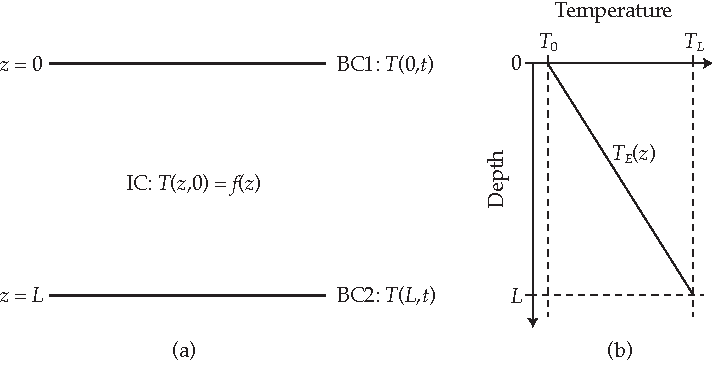
\includegraphics[]{geothermics/figures/fourier_setup.pdf}
    \caption{Model setup used to solve the 1-D, conductive, heat equation with
    fixed temperature boundary conditions and no internal heat sources.}
    \label{fig:fsetup}
\end{figure}

Another constraint we can place on the thermal evolution is the asymptotic temporal solution ($t \to \infty$). Since there are no sources in this model, the equilibrium solution, $T_E(z)$, satisfies $\pdv[2]{T_E}{z} = 0$.  We may also refer to the equilibrium solution as the steady-state solution.  For our chosen problem, the equilibrium solution is simply a linear temperature function between the fixed boundary temperatures,
\begin{equation}
    T_E(z) = T_0 + \frac{T_L - T_0}{L} z .
\end{equation}

We can define a displacement function as the difference between our desired solution and the equilibrium temperature,
\begin{equation}
    R(z,t) = T(z,t) - T_E(z) ,
    \label{eq:R}
\end{equation}
with boundary conditions $R = 0$ at $z = 0 and L$.  We can show that $\pdv{R}{t}
= \pdv{T}{t}$ and $\pdv[2]{R}{z} = \pdv[2]{T}{z}$, which means $R$ also satisfies
the heat equation,
\begin{equation}
    \pdv{R}{T} = \kappa \pdv[2]{R}{z} .
\end{equation}
It may seem like we haven't made much progress towards the solution we care about, $T(z,t)$, except that the solution to $R(z,t)$ is well known.  What we have done is turn our problem into one with differing boundary temperatures (inhomogeneous boundary conditions) to one with quite simple and equal boundary conditions (homogeneous boundary conditions).  Using a Fourier series, we can write the solution to $R(z,t)$ as
\begin{equation}
    R(z,t) = \sum_{n=1}^{\infty} a_n \sin \left( \frac{n \pi z}{L} \right)
    \exp \left( -\frac{ n^2 \pi^2 }{L^2} \kappa t \right)
    \label{eq:Rsoln}
\end{equation}
Equating~\ref{eq:R} and \ref{eq:Rsoln},
\begin{equation}
    T(z,t) - T_E(z) = \sum_{n=1}^{\infty} a_n \sin \left( \frac{n \pi z}{L} \right)
    \exp \left( -\frac{ n^2 \pi^2 }{L^2} \kappa t \right) ,
    \label{eq:Tsoln}
\end{equation}
and applying the initial condition, $T(z,0) = f(z)$, we find
\begin{equation*}
    f(z) - T_E(z) = \sum_{n=1}^{\infty} a_n \sin \left( \frac{n \pi z}{L} \right)
\end{equation*}
where the Fourier coefficients, $a_n$ are found by
\begin{equation}
    a_n = \frac{2}{L} \int_0^L [f(z) - T_E(z)] \sin \left( \frac{n \pi z}{L}
    \right) \dd{z} .
    \label{eq:fcoef}
\end{equation}

Finally, rearranging Equation~\ref{eq:Tsoln} we find
\begin{equation}
    T(z,t) =  T_E(z) + \sum_{n=1}^{\infty} a_n \sin \left( \frac{n \pi z}{L} \right)
    \exp \left( -\frac{ n^2 \pi^2 }{L^2} \kappa t \right) .
\end{equation}

Now all we need to know is the initial condition in order to find the Fourier coefficients using Equation~\ref{eq:fcoef} and to compute the temperature as the system cools.  The versatility of such a solution is the range of initial conditions that we can supply and the range of problems that can be solved.  While the problems are likely to be quite simple physically, they can still provide useful insight into the variations of temperature, heat flow, subsidence and characteristic cooling scales that we can reasonably expect for physical processes acting within the Earth.

%----------------------------------------------------------
\subsection{Half-space model}

The half-space cooling model provides one of the simplest and most widely applicable solutions to the heat equation. It describes the thermal evolution of a semi-infinite medium that undergoes a sudden change in surface temperature. Because no intrinsic length scale is imposed, the solution depends only on the combined variable $\eta = z / (2\sqrt{\kappa t})$, reflecting the diffusive nature of heat transport.

This model is relevant to a wide range of geophysical problems, including the cooling of newly formed oceanic lithosphere, the thermal evolution of lava flows and lava lakes before cooling reaches their base, and any situation in which heat diffuses into (or out of) a medium that is effectively infinite laterally and vertically over the timescale of interest.

\subsubsection{Derivation}

For simple half-space cooling, we assume the surface temperature is held constant and the entire Earth is at some mantle temperature.  Cooling of a half-space with constant thermal properties and no internal heat production is determined by solving the PDE discussed above,
\[
    \pdv{T}{t} = \kappa \pdv[2]{T}{z} .
\]
The boundary and initial conditions are given by
\begin{align*}
    \text{BC:} \quad T(0,t) &= T_0 , \\
    \lim_{z \to \infty} T(z,t) &= T_a , \\
    \text{IC:} \quad T(z,0) &= T_a,
\end{align*}
To solve this PDE (a function of time and space), we will turn it into an ODE (a function of one variable).  To do so, we will introduce a non-dimensional parameter and a new non-dimensional temperature,
\begin{align*}
    \eta &= z / 2 \sqrt{\kappa t} , \\
    \theta(\eta) &= \frac{T(z,t) - T_0}{T_a - T_0},
\end{align*}
which allows us to write,
\[
    -\eta \dv{\theta}{\eta} = \frac{1}{2} \dv[2]{\theta}{\eta} ,
\]
with a single boundary condition $\theta(0) = 0$.  The solution to this PDE is well known,
\[
    \theta(\eta) = \erf (\eta) ,
\]
where $\erf (x)$ is the error function,
$\frac{2}{\sqrt{\pi}}\int_0^{x} e^{-\xi^{2}} \dd{\xi}$ (Box~\ref{box:erf}).

Next, we merely substitute for our non-dimensional parameters and solve for the temperature function,
\begin{equation}
T(z,t) = T_0 + (T_a - T_0) \erf \left( \frac{z}{2 \sqrt{\kappa t}} \right),
\end{equation}

\begin{figure}[hbtp]
    \centering
    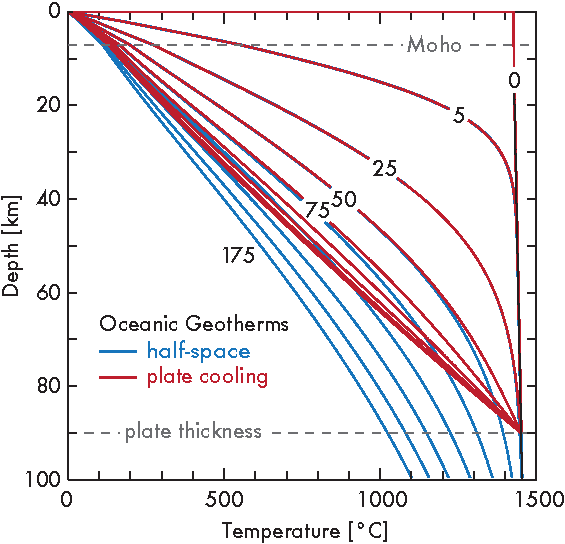
\includegraphics[]{geothermics/figures/oceanic_geotherms.pdf}
    \caption{Temperature solutions to the 1-D half-space and plate cooling
    models applicable to the oceanic lithosphere.}
    \label{fig:og}
\end{figure}

For transient problems, the surface heat flow is not constant but can be calculated as a function of time using Fourier's Law,
\begin{equation}
    q_{0}(t) = \frac{k (T_{a} - T_{0})}{\sqrt{\pi \kappa t}}.
\end{equation}

%Rocks, like most materials, expand when heated (or contract when cooled) and
%experience a change in density as a result
%\begin{equation}
%    \rho(T) = \rho_0 [1 + \alpha (T - T_0)],
%\end{equation}
%where $\rho_0$ is the reference density, measured at the reference temperature,
%T_0$.

Rocks, like most materials, expand when heated (or contract when cooled) and as a result, experience a change in density.  This change in density affect the overall buoyancy of the lithosphere and using the principles of isostasy we can solve for this subsidence.

The subsidence, $s$, is a little more difficult to compute (since it involves integration) but arises from balancing isostatic columns.  The density variations result from the thermal contraction the lithosphere and the in-filling density of water above the cooler column.  Subsidence can be computed using
\begin{equation}
    s(t) = \frac{\rho_{m}}{\rho_{m} - \rho_{w}} \alpha
        \int_{0}^{\infty} [ T(z,0) - T(z,t) ] \dd{z},
    \label{eq-subsidence}
\end{equation}
where $\rho_{w}$ and $\rho_{m}$ are seawater and mantle density, respectively.  The volumetric expansivity is given by $\alpha$, and the initial geotherm is $T(z,0)$.  Temperature is integrated from the surface to the depth of compensation, which is infinite in the case of a half-space.  The subsidence for half-space cooling is given by
\begin{equation}
    s(t) = \frac{2 \rho_{m} \alpha (T_{m} - T_{0})}
        {(\rho_{m} - \rho_{w})}\sqrt{\frac{\kappa t}{\pi}}.
\end{equation}
\begin{figure}[hbtp]
    \centering
    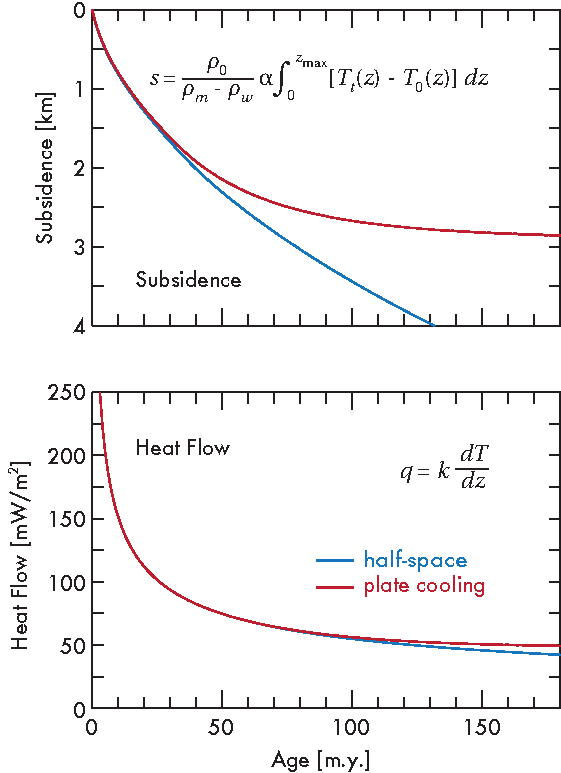
\includegraphics[]{geothermics/figures/oceanic_tis.pdf}
    \caption{Subsidence and heat flow as a function of age.}
    \label{fig:otis}
\end{figure}

\subsubsection{Thermal Length and Diffusion Time}
Often in physics, we try to make estimates for some scale (e.g.\ distance, time) related to a process without having to perform (or in advance of) an experiment.

For transient thermal processes we can examine the argument of the error function.  The argument of the error function must be unitless (much like the arguments of $\exp$, $\log$, and trigonometric functions).  We define one thermal length when the argument of the error function is equal to 1 (i.e., $\erf (1)$).  Hence the thermal length is given by
\begin{equation}
  z = 2 \sqrt{\kappa t},
\end{equation}
and represents the depth at which $\sim$16\% of the change in temperature from $T_{a}$ to $T_0$ is observed.  We can also use this relationship to estimate the time at which the propagating thermal wave can be felt at a given distance from the temperature perturbation,
\begin{equation}
    t = \frac{z^2}{4 \kappa} ,
\end{equation}
wich is know as the diffusion or characteristic time.

% ----- Error function -----
\ntextbox{Error Function}{
    The error function derives its name from applications in probability and statistics.  However, the error function is a common within many solutions to the heat equation.  The error function is defined as
    \begin{equation*}
        \erf (x) = \frac{2}{\sqrt{\pi}}\int_{0}^{x} e^{-\xi^{2}} \dd{\xi}.
    \end{equation*}
    The error function is an odd function (i.e.\ $\erf (-x) = - \erf (x))$ where
    \begin{align*}
        \erf (0) & = 0 \\
        \lim_{x \to \infty} \erf (x) = 1.
    \end{align*}

    Some solutions to the heat equation require the complementary error function,
    \begin{align*}
        \erfc (x) & = 1 - \erf(x) \\
        \erf (x) & = \frac{2}{\sqrt{\pi}}\int_{x}^{\infty} e^{-\xi^{2}} \dd{\xi}.
    \end{align*}

    We typically use the point at which the argument of the error function is equal to unity (i.e.\ $\erf (1)$) to estimate parameters such as the time it takes to cool to a given depth or the depth cooling has reached in a given time.  At $\erf (1) \approx 0.8427$, 16\% of the temperature step has occurred.

    \begin{center}
        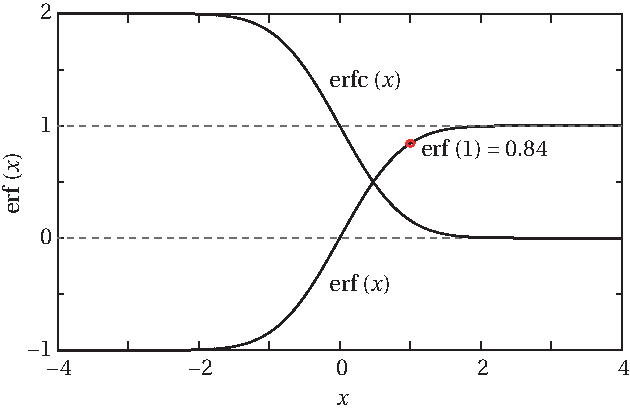
\includegraphics[]{geothermics/figures/erf.eps}
        \captionof{figure}{The error function and its complement.}
        \label{fig:erf}
    \end{center}

    The error function is reasonably linear to an argument of $\sim$0.75 and then rapidly asymptotes towards 1.  By an argument of 3, the result is 0.9999779\ldots.
    \begin{center}
    \captionof{table}{The error function values as a function of the argument.}
    \label{tab:erf}
    \begin{tabular}{@{}cccccc@{}}
        \toprule
        \textbf{argument}, $x$ & $\erf(x)$ & $\erfc(x)$ & $x$ & $\erf(x)$ & $\erfc(x)$ \\
        \midrule
        -3.0000 &  $\sim$-1.0000 &  $\sim$2.0000 &   0 &  0       &   1.0000 \\
        -2.5000 &  -0.9996 &   1.9996 &   0.1000  &  0.1125  &   0.8875 \\
        -2.0000 &  -0.9953 &   1.9953 &   0.2000  &  0.2227  &   0.7773 \\
        -1.7500 &  -0.9867 &   1.9867 &   0.3000  &  0.3286  &   0.6714 \\
        -1.5000 &  -0.9661 &   1.9661 &   0.4000  &  0.4284  &   0.5716 \\
        -1.2500 &  -0.9229 &   1.9229 &   0.5000  &  0.5205  &   0.4795 \\
        -1.0000 &  -0.8427 &   1.8427 &   0.6000  &  0.6039  &   0.3961 \\
        -0.9000 &  -0.7969 &   1.7969 &   0.7000  &  0.6778  &   0.3222 \\
        -0.8000 &  -0.7421 &   1.7421 &   0.8000  &  0.7421  &   0.2579 \\
        -0.7000 &  -0.6778 &   1.6778 &   0.9000  &  0.7969  &   0.2031 \\
        -0.6000 &  -0.6039 &   1.6039 &   1.0000  &  0.8427  &   0.1573 \\
        -0.5000 &  -0.5205 &   1.5205 &   1.2500  &  0.9229  &   0.0771 \\
        -0.4000 &  -0.4284 &   1.4284 &   1.5000  &  0.9661  &   0.0339 \\
        -0.3000 &  -0.3286 &   1.3286 &   1.7500  &  0.9867  &   0.0133 \\
        -0.2000 &  -0.2227 &   1.2227 &   2.0000  &  0.9953  &   0.0047 \\
        -0.1000 &  -0.1125 &   1.1125 &   2.5000  &  0.9996  &   0.0004 \\
        0       &  0.0000  &   1.0000 &   3.0000  &  $\sim$1.0000  &   $\sim$0.0000 \\
        \bottomrule
    \end{tabular}
\end{center}
}{mathtool}\label{box:erf}

\subsection{Plate Cooling}

While the half-space solution provides a useful first-order description of lithospheric cooling, it does not reproduce the observed long-term behaviour of the ocean basins. In particular, both seafloor subsidence and surface heat flow decrease rapidly at young ages but tend to level off in older lithosphere. This flattening suggests that cooling is limited by a process not captured by the half-space model.

An alternative framework, proposed by \citet{McKenzie1967}, is the plate cooling model. The key difference between the two models lies in the basal boundary condition: the half-space model assumes an infinite domain, whereas the plate model imposes a finite lithospheric thickness with a fixed temperature at its base (Figure \ref{fig:plate}). This constraint limits the growth of the thermal boundary layer and leads to a more realistic long-term thermal evolution of oceanic plates.

This 1-D solution and the 2-D version of this problem are used to model the temperature, heat flow, and subsidence of the oceanic lithosphere. Note the spreading velocity only matters when plate velocities fall below $\sim\SI{10}{mm.a^{-1}}$, so the 1-D model is generally sufficient.
\begin{figure}[hbtp]
  \centering
  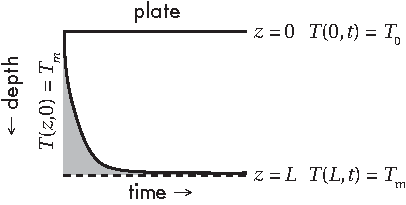
\includegraphics[]{geothermics/figures/platesetup.pdf}
  \caption{Plate model setup.}
  \label{fig:plate}
\end{figure}

\ntextbox{Derivation of Fourier Coefficients for Plate Cooling}{
    The solution consists of two parts, a constant gradient term representing the asymptotic solution and the Fourier series of a function that, when combined, the two parts give the initial condition as discussed in Section~\ref{sec:fseries} above.  The initial condition is a constant temperature throughout the plate, $f(z) = T_m$.  The equilibrium condition is a linear solution from the surface to the maximum depth of the plate $L$, 
    \[
        T_E = T_0 + (T_m - T_0)L^{-1}z .
    \]
    To find the Fourier coefficients for this problem we use Equation~\ref{eq:fcoef} and substitude in the initial and equilibrium functions,
    \begin{align*}
        a_n &= \frac{2}{L} \int_0^L \left[T_m - T_0 + \frac{T_m - T_0}{L} z \right]
        \sin \left( \frac{n \pi z}{L} \right) \dd{z} \\
        &= \frac{2}{L} \int_0^L (T_m - T_0) \left(1 + \frac{z}{L} \right)
        \sin \left( \frac{n \pi z}{L} \right) \dd{z}.
    \end{align*}
    We can break the integral up into two separate integrals to evaluate separately
    \[
        a_n = \frac{2(T_m - T_0)}{L} \Biggl(
        \underbrace{\int_0^L \sin \left( \frac{n \pi z}{L} \right)
        \dd{z}}_\text{\ding{202}} +
        \frac{1}{L}\underbrace{\int_0^L z \sin \left( \frac{n \pi z}{L} \right)
        \dd{z}}_\text{\ding{203}} \Biggr)
        .
    \]
    To solve each integral, we employ $u$-substitution with
    \begin{align*}
        u &= \frac{n \pi z}{L} \\
        \dd{u} &= \frac{n \pi}{L} \dd{z} \\
        \text{lower limit:}&\text{ at } z = 0, u = 0 \\
        \text{upper limit:}&\text{ at } z = L, u = n \pi .
    \end{align*}
    For \ding{202} the resulting integral is
    \begin{align*}
        \int_0^L \sin \left( \frac{n \pi z}{L} \right) \dd{z}
        &= \frac{L}{n \pi} \int_0^{n \pi}  \sin u \dd{u} \\
        &= \left. - \frac{L}{n \pi} \cos u \dd{u} \right|_{0}^{n \pi} \\
        &= - \frac{L}{n \pi} (\cos (n\pi) - 1) .
    \end{align*}
    Since $n$ is an integer, $\cos u$ is either -1 or 1 depending upon $n$ being either odd or even, respectively.  To say this another way, $\cos(n\pi) = (-1)^n$. And so \ding{202} becomes
    \[
        \frac{L}{n \pi}((-1)^n + 1)
    \]
    Following a similar process for \ding{203} the resulting integral is
    \begin{align*}
        \int_0^L z \sin \left( \frac{n \pi z}{L} \right) \dd{z} &= 
        \frac{L^2}{n^2 \pi^2} \int_0^{n \pi} u \sin u \dd{u} \\
        &= \frac{L^2}{n^2 \pi^2} \left. \sin u \right|_0^{n\pi} - \left. u \cos u \right|_0^{n\pi} \\
        &= \frac{L^2}{n^2 \pi^2} \sin (n\pi) - \sin 0 - (n\pi \cos(n\pi) - 0 \cos 0) \\
        &= - \frac{L^2}{n^2 \pi^2} n \pi \cos(n\pi) \\
        &= - \frac{L^2}{n \pi} (-1)^n .
    \end{align*}

    Substituting the resulting expressions from \ding{202} and \ding{203} back into $a_n$ and simplifying
    \[
        a_n = \frac{2 (T_m - T_0)}{L} \left( \frac{L}{n \pi}[(-1)^n + 1] -
        \frac{1}{L} \frac{L^2}{n \pi} (-1)^n \right)
    \]
    we find the value of the Fourier coefficients for the plate cooling model are given by
    \[
        a_n = \frac{2(T_m - T_0)}{n \pi} .
    \]
}{core}\label{box:platecooling}
\FloatBarrier

\subsubsection{Solution}
Temperatures for the plate cooling model can be estimated from the following relation,
\begin{equation}
    \workeq
    T(z,t) = T_{0} - (T_{m} - T_{0})
    \left[\frac{z}{L} + \frac{2}{\pi}\sum_{n = 1}^{\infty}
    \frac{1}{n} \sin\left(\frac{n \pi z}{L}\right)
    \exp\left(- \frac{n^2 \pi^2 \kappa t}{L^2}\right) \right].
    \label{eq:plateT}
\end{equation}
Heat flow is given by
\begin{equation}
    q_{0}(t) = k \eval{\pdv{T}{z}}_{z=0} = 
    \frac{k (T_{m} - T_{0})}{L}
    \left[ 
        1 + 2 \sum_{n = 1}^{\infty} \exp\left( -\frac{n^2 \pi^2 \kappa t}{L^2}\right)
    \right],
    \label{eq:plateq}
\end{equation}
and the subsidence is found by
\[
    s(t) = \frac{\rho_m \alpha}{\rho_m - \rho_w}\int_0^L \left[T(z,t) - T_m\right] \dd{z}
\]
which after integration of $T(z,t)$ yields
\begin{equation}
    s(t) = \frac{\rho_{m} \alpha (T_{m} - T_{0}) L}{2 (\rho_{m} - \rho_{w})}
        \left[ 1 - \frac{8}{\pi^2} \sum_{n = 0}^{\infty} \frac{1}{(2n + 1)^2}
        \exp\left( -\frac{(2n + 1)^2 \pi^2 \kappa t}{L^2} \right) \right].
    \label{eq:plates}
\end{equation}
\begin{figure}[hbtp]
  \centering
  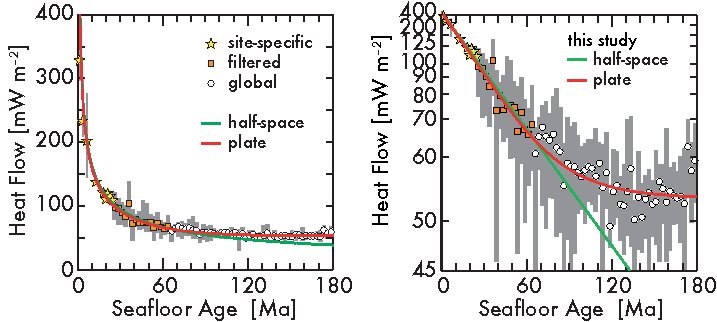
\includegraphics{geothermics/figures/hfage.pdf}
  \caption{Plate (red) and half-space (green) cooling models fit to oceanic heat flow data.  Both plots illustrate the same result with the linear scales and on the left and (heat flow)$^{-2}$ on the right to illustrate the differences between the heat flow and age relationships for the two cooling models.}
  \label{fig-hfage}
\end{figure}
While the solution to each of these is an infinite sum, we can approximate the solution by setting an acceptable tolerance for the error in the solution (or changes between successive terms within the sum).

\subsubsection{Time and Depth Scales}

The solution to the plate cooling model can be laborious to compute but we can develop two separate approximations that simplify the computations considerably.  Examining the argument of the exponential from the solution for heat flow of a plate (Equation~\ref{eq:plateq}) we can define the characteristic time as
\begin{equation}
    \tau = \frac{L^2}{\kappa},
\end{equation}
which has the units of time.

At the early-stages of cooling ($t \ll \tau$), the heat loss is essentially the same as the half-space cooling model, which can be approximated by
\begin{equation}
    q_{0}(t) \approx \frac{k (T_{m} - T_{0})}{\sqrt{\pi \kappa t}}.
\end{equation}

For late-stage cooling ($t \gg \tau$), the heat loss can be approximated by only the first term ($n = 1$) of the summed term in Equation~\ref{eq:plateq},
\begin{equation}
    q_{0}(t) \approx \frac{k (T_{m} - T_{0})}{L}
        \left[ 1 + 2 \exp\left( -\frac{\pi^2 \kappa t}{L^2}\right) \right].
\end{equation}

At very long time periods, the heat flow approaches an asymptotic value
\begin{equation}
    \lim_{t \to \infty} q_{0}(t) = \frac{k (T_{m} - T_{0})}{L}.
\end{equation}


\subsection{1-D Transient Solutions}\label{sec:fseries}

Let us consider how to solve problems such as the plate cooling model below, but for slightly more complicated cases (i.e. ones in which the temperature is not initially constant).  We will be exploring the transient heat flow equation without sources
\begin{equation}
    \pdv{T}{t} = \kappa \pdv[2]{T}{z} .
\end{equation}
The boundary and initial conditions are given by
\begin{align}
    \textbf{BC:} \quad T(0,t) &= T_0 , \\
    T(L,t) &= T_L , \\
    \textbf{IC:} \quad T(z,0) &= f(z),
\end{align}
where $f(z)$ is an arbitrary function of temperature as a function of depth.  For the plate cooling model above, $f(z) = T_L$.  We cannot solve this problem directly because the boundary conditions are not homogeneous (i.e. $T_0 \neq T_L$).  So we need to look for a way to rewrite---at least part---of this problem with homogeneous boundary conditions.

To reformulate our problem, we will subtract the equilibrium solution from the transient solution to give the problem homogeneous boundary conditions.  The equilibrium temperature distribution is given by Laplace's equation,
\begin{equation}
    \pdv[2]{T_E}{z} = 0 ,
\end{equation}
with the boundary conditions:
\begin{align}
    T_E(0) &= T_0 , \\
    T_E(L) &= T_L .
\end{align}
Since there are no sources we can easily guess the equilibrium solution,
\begin{equation}
    T_E(z) = T_0 + \frac{T_L - T_0}{L} z .
\end{equation}

To continue reformulating our problem, we will look at the transient cooling as a displacement from equilibrium.  To do this, all we need to do is define the displacement temperature as
\begin{equation}
    \theta(z,t) \equiv T(z,t) - T_E(z) .
\end{equation}
From this definition, it follows that
\begin{equation}
    \pdv{\theta}{t} = k \pdv[2]{\theta}{z} ,
\end{equation}
and subtracting the equilibrium boundary and initial conditions from those
of our original transient PDE,
\begin{align}
    \text{BC:} \quad \theta(0,t) &= 0 , \\
    \theta(L,t) &= 0 , \\
    \text{IC:} \quad \theta(z,0) &= f(z) - T_E(z) .
\end{align}

Now that we have a PDE with homogeneous boundary conditions we can solve the PDE using the standard separation of variables
\begin{equation}
    \theta(z,t) = \sum_{n=1}^\infty a_n \sin \left( \frac{n \pi z}{L} \right)
    \exp \left( - \frac{n^2 \pi^2}{L^2} \kappa t \right) .
\end{equation}
The initial conditions imply,
\begin{equation*}
    f(z) - T_E = \sum_{n=1}^\infty a_n \sin \left( \frac{n \pi z}{L} \right) ,
\end{equation*}
hence the Fourier coefficients are given by
\begin{equation}
    a_n = \frac{2}{L} 
        \int_0^L [f(z) - T_E(z)] \sin \left( \frac{n \pi z}{L} \right) \dd{z} .
\end{equation}

Now that we have solved for the Fourier coefficients we can calculate the transient cooling using our previous definition of $\theta(z,t)$
\begin{equation}
    T(z,t) = T_E(z) + \theta(z),
\end{equation}
with the full solution,
\begin{equation}
    T(z,t) = T_E(z) + \sum_{n=1}^\infty a_n \sin \left( \frac{n \pi z}{L}
    \right) \exp \left( - \frac{n^2 \pi^2}{L^2} \kappa t \right) .
\end{equation}

If the heat production is independent of time, we can also use this method to solve
\begin{equation}
    \pdv{T}{t} = \kappa \pdv[2]{T}{z} + \frac{A(z)}{\rho C_P} .
\end{equation}


\section{Cooling Involving Phase Changes}\label{sec:stefan}

Phase changes introduce latent heat into thermal problems, fundamentally altering how temperature evolves through time. Unlike purely conductive problems with fixed boundaries, latent heat problems involve \emph{moving internal boundaries} whose positions must be solved as part of the problem.

Such problems are referred to as \emph{Stefan problems} and are characterized by:
\begin{itemize}
    \item heat diffusion in each phase,
    \item a moving phase boundary,
    \item and an energy balance at that boundary that accounts for latent heat.
\end{itemize}

In this section we derive two classical examples relevant to igneous systems:
the cooling of a tabular dike and the cooling of a spherical pluton.

\subsection{Cooling of a Dike}

Consider a planar igneous dike intruded into cooler country rock. The dike
solidifies inward from its margins as heat is conducted away. We idealize the
problem as one-dimensional and symmetric about the dike center.

Let $x$ denote distance normal to the dike, with $x=0$ at the center. The solid--
liquid interface is located at $x = \pm s(t)$, where $s(t)$ is an unknown function
of time. Temperature evolves by conduction in both the solid and liquid regions,
\[
    \pdv{T}{t} = \kappa \pdv[2]{T}{x}.
\]

We impose:
\begin{align*}
    \text{BC1:}\quad T(x,0) &= T_0 \qquad \text{for } |x| < s(0), \\
    \text{BC2:}\quad T(x,t) &\rightarrow T_\infty \qquad \text{as } |x| \rightarrow \infty.
\end{align*}

The phase boundary is constrained to be at the melting temperature,
\[
    T(x = s(t)) = T_m .
\]

By symmetry,
\begin{equation}
    \eval{\pdv{T}{x}}_{x=0} = 0.
\end{equation}

The key physical constraint enters through conservation of energy at the moving
interface. As the solidification front advances, latent heat is released at a rate
proportional to the speed of the interface. This heat must be conducted away through the surrounding solid. Balancing these effects at the propagating boundary yields the Stefan condition,
\begin{equation}
    \rho L \frac{ds}{dt} = - k \eval{\pdv{T}{x}}_{x = s(t)^-},
\end{equation}
where $L$ is the latent heat of fusion per unit mass.

The coupled system admits a similarity solution in which the position of the
solidification front evolves as
\begin{equation}
    s(t) = 2 \lambda \sqrt{\kappa t},
\end{equation}
with the dimensionless constant $\lambda$ determined implicitly by the Stefan
condition. The essential result is that the interface advances proportional to
$\sqrt{t}$ rather than linearly in time. Latent heat therefore acts to slow cooling: energy extracted from the system is consumed by phase change rather than temperature reduction. The $\lambda$ parameter is not analytic, but can be determined by the transcendental equation arising from the Stefan condition:
\begin{equation}
    \workeq
    \lambda e^{\lambda^2} \erf (\lambda) = \frac{L}{C_P (T_m - T_\infty)}.
\end{equation}

The key result is that the solidification front advances as
\[
    s(t) \propto \sqrt{t},
\]
not linearly in time. Latent heat slows cooling by requiring that energy be removed
to change phase rather than temperature. Large latent heat or small temperature
contrast leads to slow crystallization.

%----------------------------------------------------------
\subsection{Cooling of a Spherical Pluton}

We now consider the solidification of a spherical pluton of radius $R$, surrounded
by cooler country rock. In contrast to the dike, curvature plays an essential role.

Let $r$ denote radial distance from the pluton center, and let $r = s(t)$ denote the solidification front.

\subsubsection*{Governing equation}

In spherical symmetry, the diffusion equation takes the form:
\begin{equation}
    \frac{\partial T}{\partial t} =
    \kappa \left( \frac{1}{r^2}\pdv{}{r} \left( r^2 \pdv{T}{r} \right) \right).
\end{equation}

\subsubsection*{Boundary and Initial Conditions}

At the center,
\begin{equation}
\left.\frac{\partial T}{\partial r}\right|_{r=0} = 0.
\end{equation}

At large distances,
\begin{equation}
T(r,t) \rightarrow T_\infty \quad \text{as } r \rightarrow \infty.
\end{equation}

The phase boundary satisfies
\begin{equation}
T\bigl(r = s(t)\bigr) = T_m.
\end{equation}

\subsubsection*{Stefan condition for a sphere}

Energy conservation at the moving boundary requires
\begin{equation}
\rho L \frac{ds}{dt} = - k \eval{ \pdv{T}{r} }_{r=s(t)^-}.
\end{equation}

The mathematical form is identical to the planar case, but the temperature gradient
now reflects spherical geometry.

\subsubsection*{Similarity form}

As in the planar Stefan problem, the solution admits a similarity form
\begin{equation}
s(t) = 2 \lambda \sqrt{\kappa t},
\end{equation}
but the value of $\lambda$ differs because the diffusion operator is different.

The solidification front again advances proportional to $\sqrt{t}$, but cooling is
more efficient than in the planar case because curvature enhances heat loss.

\subsubsection*{Comparison with the dike problem}

\begin{itemize}
\item Both problems exhibit $s(t) \propto \sqrt{t}$ behavior.
\item Latent heat controls the pace of solidification in both geometries.
\item Spherical plutons cool faster than planar dikes for the same material
properties due to geometric heat focusing.
\end{itemize}

\subsection{Metamorphic Reaction Fronts}

Metamorphic reaction fronts also release or absorb latent heat and propagate through rock, but unlike igneous solidification they are typically coupled to reaction kinetics and mass transport. Whether such fronts admit analytical solutions depends on the simplifications adopted and will be considered separately.
\begin{itemize}
    \item Show how cooling/heating rates are modified
    \item Emphasize that temperature evolution != heat flow evolution
    \item New conceptual depth without heavy math

    \item Note that the signal is superimposed on the background (solid Earth) thermal gradient
    \item Depth of penetration
    \item Timescale dependence
\end{itemize}

%----------------------------------------------------------
\section{Climatic Forcing of the Solid Earth}

Until now, we have assumed that the surface temperature of Earth is a constant value.  While this assumption is fine for the construction of crustal and lithospheric scale geotherms it is clearly not constant as we ourselves respond to the yearly and daily variations.  These atomospheric variations affect ground surface temperatures.  Ground surface temperatures vary through time on a wide range of timescales, from daily and seasonal cycles to glacial-interglacial transitions and long-term climate change.  Because the solid Earth responds to thermal forcing by diffusion, these variations propagate downward from the surface, modifying subsurface temperatures without destroying the underlying conductive structure.

In this section, we examine how surface temperature variability acts as a time-dependent boundary condition on the thermal diffusion equation, how the resulting signals decay with depth, and what geological consequences follow from these processes.

\subsection{Downward propagation of thermal signals}

The temperature evolution in the shallow crust in response to a ground surface temperature change is governed by the one-dimensional diffusion equation,
\begin{equation}
    \frac{\partial T}{\partial t} = \kappa \frac{\partial^2 T}{\partial z^2},
\end{equation}
where $z$ is depth measured downward from the surface. When surface temperature varies in time, it enters the problem as a time-dependent boundary condition,
\begin{equation}
    T(0,t) = T_s(t).
\end{equation}
The ground surface temperature variations are superimposed on top of the background thermal gradient.  Hence, it is useful to decompose the temperature field into a steady-state background geotherm and a transient perturbation,
\begin{equation}
    T(z,t) = T_\Gamma(z) + T'(z,t),
\end{equation}
where $T_\Gamma(z)$ satisfies the steady-state equation and $T'(z,t)$ represents the climatically forced signal. Because the diffusion equation is linear, these components superimpose without interacting: climatic signals modify temperatures but do not erase the background thermal gradient of the solid Earth.

A key feature of diffusion is that the depth to which a thermal signal penetrates depends on its characteristic timescale. Short-period signals are confined to shallow depths, while long-period signals diffuse more deeply. This timescale dependence is made explicit by examining a simple analytic solution.

%----------------------------------------------------------
\subsection{Surface boundary condition variability}

\subsubsection*{Periodic forcing: daily and annual thermal waves}

Consider the case of sinusoidal surface temperature forcing,
\begin{equation}
    T_s(t) = T_{\mathrm{mean}} + T_a \cos(\omega t),
\end{equation}
where $T_a$ is the amplitude and $\omega = 2\pi/\tau$ is the angular frequency associated with period $\tau$.

We seek solutions of the form
\begin{equation}
    T'(z,t) = \Re\left\{ \hat{T}(z) e^{i\omega t} \right\},
\end{equation}
which, when substituted into the diffusion equation, yields
\begin{equation}
    \frac{d^2 \hat{T}}{dz^2} - \frac{i\omega}{\kappa} \hat{T} = 0.
\end{equation}

The physically acceptable solution that decays with depth is
\begin{equation}
    T'(z,t) = T_a e^{-z/\delta} \cos\!\left(\omega t - \frac{z}{\delta}\right),
\end{equation}
where the characteristic decay length
\begin{equation}
    \delta = \sqrt{\frac{2\kappa}{\omega}} = \sqrt{\frac{\kappa \tau}{\pi}}
\end{equation}
is known as the \emph{thermal skin depth}.

This result shows explicitly where the skin-depth scaling comes from. The amplitude of the temperature signal decays exponentially with depth, and the phase of the signal is delayed in proportion to depth. Both effects are controlled entirely by thermal diffusivity and the forcing period.

For diurnal forcing, the skin depth is of order tens of centimeters; for annual forcing, it is several meters. These shallow depths reflect the short timescales of the imposed surface variability.

\subsubsection*{Recent climate change}

Surface temperature changes associated with recent climate change act on decadal to
centennial timescales, corresponding to skin depths of hundreds of meters. Although
the surface perturbation is small compared to absolute temperatures at depth, its
signature can be resolved by subtracting the background geotherm.

This motivates the definition of a reduced temperature,
\begin{equation}
T_r(z,t) = T(z,t) - T_\Gamma(z),
\end{equation}
which isolates the transient climatic signal. Reduced temperature profiles measured
in boreholes provide a direct record of recent surface temperature history.

\subsection{Step changes in surface temperature}

While periodic forcing is useful for developing intuition, most climatic changes of geological interest are better approximated as step changes in surface temperature.  Examples include rapid post-glacial warming or abrupt climatic transitions inferred from proxy records. Step forcing leads to solutions that differ qualitatively from sinusoidal thermal waves and form the basis of most paleoclimate corrections applied to borehole data.

We consider the one-dimensional diffusion equation,
\begin{equation}
    \pdv{T}{t} = \kappa \pdv[2]{T}{z},
\end{equation}
with a surface boundary condition representing an instantaneous temperature change at time $t=0$,
\begin{equation}
    T(0,t) =
    \begin{cases}
        T_\Gamma, & t < 0, \\
        T_\Gamma + \Delta T, & t \ge 0.
    \end{cases}
\end{equation}
We seek the reduced temperature
\begin{equation}
    T_r(z,t) = T(z,t) - T_\Gamma(z),
\end{equation}
which isolates the transient perturbation relative to the steady background geotherm.

\subsubsection*{Green's function solution}

The solution for a step change in surface temperature can be constructed from the
fundamental solution (Green's function) of the diffusion equation. For an impulsive
surface temperature change, the reduced temperature at depth is
\begin{equation}
    T_r(z,t) = \Delta T \, \erfc \!\left( \frac{z}{\sqrt{4\kappa t}} \right),
\end{equation}
where $\operatorname{erfc}$ is the complementary error function.

This expression gives the instantaneous response to a permanent surface temperature
offset but does not yet represent the form typically used in paleoclimate studies,
which consider the *integrated* effect of the imposed surface step.

Integrating the surface forcing in time yields the physically relevant solution for a persistent step change,
\begin{equation}
    T_r(z,t) =
    \Delta T
    \left[ (1 + 2\xi^2)\,\erfc (\xi) - \frac{2\xi}{\sqrt{\pi}} e^{-\xi^2} \right],
    \qquad
    \xi = \frac{z}{\sqrt{4\kappa t}}.
\end{equation}
This expression is the forward kernel commonly used in borehole paleoclimate analysis.  It decays smoothly with depth and exhibits a characteristic curvature that depends explicitly on the time since the surface temperature change.

\subsubsection*{Penetration depth and timescale}

The argument of the error function makes clear that the relevant nondimensional depth is
\begin{equation}
    \xi = \frac{z}{\sqrt{4\kappa t}},
\end{equation}
from which the thermal penetration depth follows immediately as
\begin{equation}
    \delta \sim \sqrt{\kappa t}.
\end{equation}
This scaling is consistent with the skin depth derived for periodic forcing, but here it arises from the transient diffusion of a step boundary condition rather than a thermal wave.

\subsubsection*{Ice ages and interglacials}

Glacial-interglacial cycles act over timescales of $10^4$--$10^5$ years and therefore penetrate kilometers into the crust. Ice is an especially effective thermal boundary condition because it both fixes surface temperature near the pressure-melting point and persists long enough for diffusion to transmit the signal deeply.

As a result, glaciated regions retain a thermal memory of past ice cover long after deglaciation, influencing present-day geothermal gradients and shallow crustal temperatures.

\subsection{Paleoclimate corrections to geotherms}

Because borehole temperatures are influenced by past surface conditions, steady-state geotherms inferred from shallow temperature data must often be corrected for paleoclimate effects. The goal of such corrections is not to infer the full climate history, but to remove its influence in order to recover the underlying conductive geotherm.

This is accomplished by modeling surface temperature history as a series of step changes or continuous variations, computing the resulting transient temperature field using the diffusion equation, and subtracting this transient from the observed temperature profile. The corrected profile then more accurately reflects present-day heat flow and lithospheric structure.

Paleoclimate corrections work because diffusion preserves linearity and superposition: the temperature field retains a separable memory of boundary condition changes that can be modeled independently of the steady background state.

\subsection{Paleoclimate series of steps}

Real climatic histories are not single step changes but sequences of warming and cooling events. Because the diffusion equation is linear, the response to an arbitrary surface temperature history can be constructed by superposition of individual steps.

Suppose the surface temperature history is approximated as a series of step changes $\Delta T_i$ occurring at times $t = \tau_i$ before present. The reduced temperature profile is then
\begin{equation}
    T_r(z) = \sum_i \Delta T_i \, G\!\left( \frac{z}{\sqrt{4\kappa \tau_i}} \right),
\end{equation}
where $G(\xi)$ is the step-response kernel,
\begin{equation}
    G(\xi) =
    (1 + 2\xi^2)\,\erfc (\xi) - \frac{2\xi}{\sqrt{\pi}} e^{-\xi^2}.
\end{equation}

Each step contributes a smooth, depth-dependent temperature anomaly whose amplitude and curvature depend on the magnitude of the surface change and the time elapsed since it occurred. Older climatic events influence deeper temperatures, while recent events dominate the shallow profile.

\subsubsection*{Connection to inverse methods}

In paleoclimate reconstruction from borehole data, the step amplitudes $\Delta T_i$ and their ages $\tau_i$ may be treated as unknown parameters. Linearization of the forward model yields a Jacobian matrix whose columns correspond to partial derivatives of $T_r(z)$ with respect to these parameters.

Because the kernel $G(\xi)$ is analytic and smooth, its derivatives can be computed explicitly, enabling efficient Newton or Gauss-Newton inversion. The resulting inverse problem is moderately ill-posed, reflecting the diffusive smoothing inherent in the physics, but remains robust when regularized appropriately.

\subsection{Interpretation}

Step-change solutions emphasize several physically important points. Thermal diffusion strongly smooths surface temperature history, limiting temporal resolution at depth.  The subsurface retains a memory of past climates, but that memory degrades systematically with both depth and time. Paleoclimate corrections therefore recover broad temperature trends rather than sharp events.

From a conceptual standpoint, surface temperature history acts as a boundary control on a diffusive system, reinforcing the view of temperature as a state variable that integrates past forcing rather than responding instantaneously.

\subsection{Geological consequences}

Surface temperature variability has geological consequences despite its shallow expression. Permafrost formation and degradation are governed by the competition between climatic forcing and diffusive heat transport, linking ground ice stability directly to timescale.

Glacial-interglacial transitions also modify subsurface temperatures beneath ice sheets, altering geothermal gradients and interacting with glacial loading and unloading.  Although mechanical effects dominate isostatic responses, thermal diffusion controls the evolution of temperature-dependent material properties in the shallow crust.

More broadly, surface temperature variability produces a non-steady shallow thermal structure that departs systematically from steady-state geotherms. This reinforces several core concepts developed earlier in the chapter: temperature is a state variable, transient signals are diffusive rather than advective, and the system retains memory of past boundary conditions.

Climatic forcing therefore provides a powerful, intuitive example of diffusion in action, linking surface processes to subsurface thermal structure and emphasizing the time-dependent nature of the solid Earth's thermal state.

\section{Sedimentation and Erosion as Transient Thermal Forcing}

In addition to changes in surface temperature, vertical motion of the Earth's surface itself introduces transient thermal effects. Sedimentation buries isotherms and tends to suppress near-surface thermal gradients, while erosion exhumes warmer material and steepens them. These effects are well documented in marine and continental settings and were analyzed classically by \citet{VonHerzen&Uyeda1963}, who showed that sediment accumulation can significantly bias heat-flow measurements if not accounted for.

Unlike climatic forcing, sedimentation and erosion modify the thermal structure not by changing temperature at a fixed boundary, but by translating the boundary through the temperature field. This distinction makes them especially instructive examples of diffusion-controlled transients.

\subsection{Problem formulation}

Consider one-dimensional heat conduction in a medium undergoing vertical motion at a constant rate $v$, positive for sedimentation and negative for erosion. In a reference frame fixed to the solid Earth, the temperature obeys
\begin{equation}
\frac{\partial T}{\partial t}
=
\kappa \frac{\partial^2 T}{\partial z^2}
-
v \frac{\partial T}{\partial z},
\end{equation}
where the final term represents advection of isotherms due to surface motion.

Equivalently, the problem may be formulated as pure diffusion with a moving surface boundary,
\begin{equation}
z_s(t) = v t,
\end{equation}
on which temperature is fixed.

These two descriptions are mathematically equivalent and emphasize that sedimentation and erosion are fundamentally kinematic boundary-condition problems rather than internal heat-source effects.

\subsection{Thermal effect of steady sedimentation}

For steady sedimentation, new material is added at the surface with temperature $T_s$. Initially, the subsurface temperature field corresponds to a steady geotherm.  As sediment accumulates, isotherms are buried faster than diffusion can restore the steady gradient.

The characteristic competition is between:
\begin{itemize}
\item the burial timescale $\tau_b = z / v$, and
\item the diffusive timescale $\tau_d = z^2 / \kappa$.
\end{itemize}

Thermal effects become significant when $\tau_b \lesssim \tau_d$, or equivalently when
\begin{equation}
v \gtrsim \frac{\kappa}{z}.
\end{equation}

Under these conditions, the near-surface thermal gradient is reduced relative to the steady-state value, and heat flow inferred from shallow measurements is systematically underestimated. This mechanism explains many of the anomalously low heat-flow values observed in rapidly sedimenting marine basins \citep{VonHerzen&Uyeda1963}.

\subsection{Erosion and exhumation}

Erosion produces the opposite effect. Removal of material exposes warmer isotherms, steepening the near-surface thermal gradient. During rapid exhumation, heat flow measured near the surface may be transiently elevated even though the deep thermal structure remains unchanged.

From a thermal perspective, erosion is the time-reverse of sedimentation: the same governing equations apply, but with $v < 0$. This symmetry emphasizes that the thermal response depends on rates and timescales rather than on the geological process itself.

\subsection{Implications for heat-flow measurements}

Sedimentation and erosion directly affect the interpretation of heat-flow data because measurements are typically made over the upper few to tens of meters, precisely where these transient effects are strongest. Without correction, shallow gradients may not represent the long-term conductive heat flow.

Von Herzen and Uyeda demonstrated that even modest sedimentation rates can suppress measured heat flow for timescales comparable to the accumulation history. The thermal structure retains a memory of sedimentation that decays only diffusively, much like climatic forcing.

\subsection{Interpretive perspective}

Sedimentation and erosion reinforce several central ideas developed in this chapter.  Thermal structure reflects not only present conditions but the integrated history of boundary motion. Temperature is a state variable with finite memory. And observed heat flow must be interpreted in light of geological context rather than treated as a direct probe of deep thermal structure.

Together with climatic forcing, sedimentation provides a compelling demonstration that many apparent heat-flow anomalies arise not from anomalous heat sources, but from transient processes acting at the Earth's surface.

\subsection{Analytic solutions for sedimentation and erosion}

The thermal effects of sedimentation and erosion can be quantified analytically for simple cases. These solutions make explicit how vertical surface motion biases temperature gradients and heat-flow estimates.

\subsubsection*{Steady sedimentation or erosion}

Consider steady sedimentation or erosion at a constant vertical rate $v$, with $v>0$ for sedimentation and $v<0$ for erosion. In a reference frame fixed to the solid Earth, temperature satisfies the advection--diffusion equation
\begin{equation}
\frac{\partial T}{\partial t}
=
\kappa \frac{\partial^2 T}{\partial z^2}
-
v \frac{\partial T}{\partial z}.
\end{equation}

In the long-time limit, the system approaches a steady state in which temperature depends only on depth. The solution for the geothermal gradient is
\begin{equation}
    \frac{dT}{dz} =
    \left(\frac{q_0}{k}\right) \exp\!\left(-\frac{v z}{\kappa}\right),
\end{equation}
where $q_0$ is the true conductive heat flow at depth. The apparent heat flow inferred from a gradient measured at depth $z$ is therefore
\begin{equation}
    q_{\mathrm{app}}(z) = q_0 \exp\!\left(-\frac{v z}{\kappa}\right).
\end{equation}

For sedimentation ($v>0$), shallow gradients are suppressed and heat flow is systematically underestimated. For erosion ($v<0$), gradients are enhanced and heat flow is overestimated. The effect grows exponentially with burial or exhumation depth.

\subsubsection*{Transient onset of sedimentation}

More commonly, sedimentation begins at some finite time in the past. Suppose that steady sedimentation at rate $v$ begins at time $t=0$, applied to an initially steady geotherm. The resulting temperature anomaly relative to the original geotherm is
\begin{equation}
    T'(z,t) = -\frac{q_0}{k} \frac{\kappa}{v}
    \left[
    \exp\!\left(-\frac{v z}{\kappa}\right)
    \erfc\!\left( \frac{z - v t}{2\sqrt{\kappa t}} \right) -
    \erfc \!\left( \frac{z}{2\sqrt{\kappa t}} \right)
    \right].
\end{equation}

At early times, the disturbance is confined to shallow depths. As time increases, the burial signal propagates downward diffusively, while the exponential factor imposes the characteristic suppression of gradients associated with steady motion.

\subsubsection*{Finite sedimentary layer emplacement}

Sedimentary basins are often better approximated by emplacement of a sedimentary layer of thickness $H$ over a finite interval. If a layer of thickness $H$ is added instantaneously with surface temperature $T_s$, the resulting temperature anomaly is equivalent to a downward translation of the thermal field,
\begin{equation}
T'(z,t) =
T_0(z-H,t) - T_0(z),
\end{equation}
with subsequent diffusion smoothing the perturbation on the timescale $t \sim H^2/\kappa$.

This formulation highlights that sedimentation and erosion primarily act by translating existing thermal structure rather than generating new heat.

\subsubsection*{Interpretive implications}

These solutions make clear why sedimentation and erosion must be accounted for when interpreting heat-flow measurements. Even modest rates can distort shallow gradients over geological timescales. The thermal imprint of surface motion decays only diffusively, leaving a memory that persists long after sedimentation or erosion ceases.

Sedimentation and erosion therefore represent a third major class of transient thermal forcing, alongside surface temperature change and latent heat, completing the conceptual framework developed in this chapter.

%----------------------------------------------------------
\section{Non-Uniqueness and Interpretation}

The preceding sections demonstrate that a wide range of thermal models can satisfy the same set of surface observations. This non-uniqueness is not a deficiency of geothermics, but a fundamental consequence of diffusion, limited data, and incomplete knowledge of subsurface structure. Interpretation therefore requires explicit recognition of trade-offs and the incorporation of independent geological constraints.

\subsection{Trade-offs}

Perhaps the most common trade-off in geothermics is between heat production and thermal conductivity. A given surface heat flow can be explained by high internal heat production combined with high conductivity, or by lower heat production paired with low conductivity. Because surface heat flow constrains only the integrated thermal resistance and internal heating, these effects cannot be uniquely separated from thermal data alone.

A related ambiguity exists between boundary conditions and internal sources. Changes in basal mantle temperature can produce thermal effects similar to those caused by variations in crustal heat production. Likewise, transient surface temperature changes may alter shallow gradients in ways that mimic changes in material properties.

Global datasets of heat flow, crustal structure, and radiogenic element distribution provide critical constraints and reduce the range of acceptable models. However, these datasets do not eliminate ambiguity. \emph{These global datasets reduce ambiguity, but do not eliminate it.} This limitation reinforces three central themes: inversion is inherently non-unique, geological information is essential, and even the best global compilations must be interpreted cautiously.

\subsection{Role of geological constraints}

Because geothermics alone cannot determine unique subsurface structure, interpretation must be guided by independent geological constraints. Lithology controls thermal conductivity and heat production; tectonic history influences lithospheric thickness and basal temperature; and petrology governs phase changes and rheological behavior.

This role for geology mirrors that in gravity and magnetic interpretation. In all potential-field methods, physics constrains admissible solutions, but geology selects among them. Model credibility arises not from mathematical optimality alone but from consistency with known structure, composition, and tectonic evolution.

Seen in this light, thermal models are best understood not as definitive solutions, but as physically plausible realizations conditioned by both observations and geological reasoning.

\section{Forward Modeling and Numerical Methods}

Throughout this chapter, analytic solutions have played a central role. They clarify physical mechanisms, reveal scaling relationships, and provide benchmarks against which more complex models can be tested. At the same time, their limitations point directly toward numerical methods.

Analytic solutions---steady-state geotherms, Stefan problems, and transient surface forcing---establish essential intuition. They demonstrate how curvature reflects internal heat sources, how moving boundaries arise from latent heat, and how thermal signals diffuse with time. These solutions also provide reference cases for validating numerical implementations.

Most geological situations of interest involve complex geometry, spatially variable properties, nonlinear rheology, or coupled processes that cannot be treated analytically. In such cases, forward modeling using finite differences or related numerical methods becomes necessary.

The governing equations introduced here carry over directly: the diffusion equation, appropriate boundary conditions, and conservation laws remain unchanged. What changes is how they are solved.

Analytic solutions are necessarily idealized. They assume simple geometry, linear material behavior, and often constant properties. While invaluable for understanding, they cannot capture many important aspects of real Earth systems. A full treatment of numerical methods is therefore deferred to Chapter~\ref{ch:finitediff}, where these limitations are addressed explicitly.

\section{Concluding Remarks}

Geothermics occupies a distinctive position among geophysical methods. Its governing equations are time-dependent, its signals diffuse rather than propagate, and its memory of past conditions decays systematically with time and depth. These characteristics shape both what can be measured and how it must be interpreted.

The methods developed in this chapter provide a foundation for forward modeling and inversion using finite differences. They also establish natural connections to other fields. Temperature influences rheology and therefore lithospheric strength. It controls electrical conductivity, linking geothermics to electromagnetic methods. It determines magnetic mineral stability through the Curie temperature, coupling thermal structure to magnetic observations.

Geothermics thus serves not only as a tool for estimating temperatures, but as a bridge linking physical processes, geological history, and multiple geophysical observables within a unified framework.

\ntextbox{Comparison of potential fields}{
    In \emph{gravity}, present-day density contrasts and structure dominate the signal, and geological history is expressed indirectly through the architecture of the crust and isostatic response. In \emph{magnetics}, history is often more explicitly recorded through remanence, mineralogical state, and alteration, allowing evolutionary processes to be resolved in ways not possible with gravity alone. In \emph{geothermics}, geometry-based models explain mean thermal structure well, but spatial and temporal variations reflect diffusion, boundary conditions, and active processes, with memory that decays systematically over time and depth.  \emph{Electrostatics} differs from gravity, magnetics, and geothermics in that it is commonly implemented as an active-source technique, providing a conceptual bridge from passive potential-field methods to time-dependent electromagnetic geophysics.

    We can summarize these differences as:
    \begin{enumerate}
        \item \textbf{Gravity}
        \begin{description}
            \item[Governing equation:] elliptic (Poisson / Laplace)
            \item[Response:] instantaneous
            \item[Time dependence:] none
            \item[Memory:] none
            \item[Source:] passive
            \item[History:] appears only insofar as it has produced present-day density structure or in decaying isostatic disequilibrium
        \end{description}

        \item \textbf{Magnetics}
        \begin{description}
            \item[Governing equation:] elliptic (Poisson / Laplace, static limit)
            \item[Response:] instantaneous
            \item[Time dependence:] none in the field
            \item[Memory:] none in the field, but may exist in the source (remanence)
            \item[Source:] passive
            \item[History:] can be encoded directly in remanent magnetization (paleomagnetism)
        \end{description}

        \item \textbf{Geothermics}
        \begin{description}
            \item[Governing equation:] parabolic (diffusion) in general
            \item[Response:] intrinsic time-dependent
            \item[Memory:] finite and decaying
            \item[\emph{Long-time limit:}] reduces to an elliptic (steady-state) problem
            \item[Source:] passive
            \item[History:] transiently through thermal anomalies; persistently through boundary conditions and internal heat sources
        \end{description}

        \item \textbf{Electrostatics}
        \begin{description}
            \item[Governing equation:] elliptic (Poisson / Laplace)
            \item[Response:] instantaneous
            \item[Time dependence:] none in the static limit
            \item[Memory:] none in the field
            \item[Source:] active / passive
            \item[History:] expressed only through present-day conductivity structure or natural source terms (self-potential); most applications rely on imposed active sources
        \end{description}
    \end{enumerate}
}{aside}

\clearpage
\nocite{Beardsmore&Cull2001}
\nocite{Carslaw&Jaeger1986}
\nocite{Fowler1990}
\nocite{Jaupart&Mareschal2011}
\nocite{Lowrie1997}

\bibliographystyle{elsarticle-harv}
\bibliography{ref}